\documentclass[11pt, twocolumn]{article}

\usepackage[spanish]{babel}
\usepackage[none]{hyphenat}
\usepackage[left=1.5cm, right=1.5cm, top = 2cm, bottom=2.5cm]{geometry}
\usepackage{enumitem}
\usepackage{longtable}
\usepackage{multirow, makecell}
\usepackage{listings}
\usepackage{color}
\usepackage{graphicx}
\usepackage{subcaption}
\usepackage{parskip}
\usepackage[hidelinks]{hyperref}
\usepackage{fancyhdr}
\usepackage[export]{adjustbox}

\newcommand{\linejump}{\hfill \break}
\renewcommand{\thefootnote}{\fnsymbol{footnote}}

\definecolor{dkgreen}{rgb}{0,0.6,0}
\definecolor{gray}{rgb}{0.5,0.5,0.5}
\definecolor{mauve}{rgb}{0.58,0,0.82}
\lstset{
    language=Java,
    aboveskip=3mm,
    belowskip=3mm,
    showstringspaces=false,
    columns=flexible,
    basicstyle={\scriptsize\ttfamily},
    numbers=none,
    numberstyle=\tiny\color{gray},
    keywordstyle=\color{blue},
    commentstyle=\color{dkgreen},
    stringstyle=\color{mauve},
    breaklines=true,
    breakatwhitespace=true,
    tabsize=3
}

\sloppy
\setlength{\parindent}{0cm}
\setlength{\columnsep}{0.5cm}
\decimalpoint
\graphicspath{{img/}}

\hypersetup{colorlinks=true, urlcolor=blue, citecolor=blue}
\urlstyle{same}

\pagestyle{fancyplain}
\fancyhf{}
\fancyhead[L]{\scriptsize 
    Universidad Nacional Autónoma de México \\
    Laboratorio de Programación Orientada a Objetos \\
    M.C. Leonardo Ledesma Dominguez
}
\fancyhead[R]{\thepage}


\begin{document}
    \twocolumn[
        \centering
        Acosta Porcayo Alan Omar, Gutiérrez Grimaldo Alejandro, Medina Villa Samuel

        \linejump

        \LARGE \textbf{Práctica 1. Entorno y Lenguaje de Programación} \\
        
        \linejump
    ]

    \section*{Resumen}
    En esta práctica tendrá como objetivo familiarizarse y probar el entorno de ejecución y el lenguaje de programación java. Para ello se llevarán a cabo actividades para entender y experimentar los conceptos básicos del lenguaje de programación orientado a objetos, como clases, objetos, métodos y atributos, todo esto con el fin de resolver ciertos problemas empleando la sintaxis básica del lenguaje, incluyendo la notación adecuada, palabras reservadas y la incorporación de comentarios para documentar el código.

    \footnotetext{
        \scriptsize 
        Acosta Porcayo Alan Omar Ing. en Computación 320206102 \\
        Gutiérrez Grimaldo Alejandro Ing. en Computación 320282098 \\
        Medina Villa Samuel Ing. en Computación 320249538
    }

    \section*{Introducción}
    Una comprensión completa de la programación orientada a objetos se logra al poner en práctica los conceptos teóricos en un lenguaje de programación real. En esta introducción, vamos a explorar los pasos clave para comenzar a programar en un lenguaje orientado a objetos. Abordaremos aspectos esenciales, como el entorno de trabajo, las herramientas disponibles y la importancia de practicar la programación para un aprendizaje efectivo.

    \subsection*{Explorando Java como Ejemplo de Lenguaje de Programación}
    Un ejemplo práctico de lenguaje orientado a objetos es Java. Fue presentado por primera vez en 1995 por Sun Microsystems, que actualmente es propiedad de Oracle. Java se destaca por ser un lenguaje de alto nivel que combina elementos de los lenguajes C y C++. Sin embargo, lo que lo hace distintivo es su enfoque en la programación orientada a objetos. Una característica única de Java es su capacidad para ser compilado e interpretado, lo que lo convierte en una herramienta versátil para el desarrollo de software.

    \subsection*{El Mundo de Java: Plataforma y Estructura}
    El mundo de Java consta de dos componentes fundamentales: la JVM (Máquina Virtual Java) y la API (Interfaz de Programación de Aplicaciones Java). La JVM permite ejecutar programas Java al simular una ``máquina virtual'' independiente con su propio sistema operativo y hardware virtual. La API proporciona componentes predefinidos que hacen que el desarrollo y la implementación de aplicaciones sean más sencillos.
    
    \subsection*{Construyendo Programas en Java}
    En el contexto de Java, los programas se organizan en clases, que se escriben en archivos de texto con la extensión .java. Estos archivos luego se compilan en archivos binarios con extensión .class, que son independientes de la arquitectura. Durante la ejecución, la JVM interpreta los archivos .class y los traduce en instrucciones ejecutables para el sistema operativo.
    
    \fancyfoot{}

    \subsection*{Herramientas de Desarrollo y Proceso de Compilación}
    Para el desarrollo en Java, el Java Development Kit (JDK) proporciona las herramientas esenciales. La compilación de archivos .java se realiza mediante el comando ``javac'' del JDK. Una vez compilado, el programa se puede ejecutar usando el comando ``java'', seguido por el nombre de la clase principal que contiene el método ``main()''.

    \subsection*{El Papel de los Entornos de Desarrollo Integrado (IDE)}
    Aunque es posible desarrollar programas utilizando un simple editor de texto y las herramientas del JDK, los Entornos de Desarrollo Integrado (IDE) ofrecen interfaces más amigables. Estos IDEs aprovechan las herramientas del JDK para simplificar y agilizar todas las etapas del desarrollo, desde escribir el código hasta ejecutarlo.
    
    \section*{Objetivos}
    \begin{itemize}
        \item Configurar y preparar un entorno de desarrollo Java en la computadora incluyendo la instalación del kit de desarrollo de Java (JDK) y un IDE.
        \item Crear un programa simple utilizando Java que demuestre la comprensión de los conceptos básicos de la programación orientada a objetos, como clases, objetos, métodos y propiedades.
        \item Utilizar bibliotecas estándar de Java para realizar tareas comunes, como entrada/salida de datos 
        \item Utilizar bucles como \textit{for} y \textit{while} para repetir acciones en el código.
    \end{itemize}

    \section*{Metodología} 
    \subsection*{Ejercicio realizado por el profesor}
    Programa que crea una escalera usando el símbolo * de de base aleatoria entre 1 y 10. 
    
    \textbf{Código}
    \begin{lstlisting}
import java.util.Random;

public class MiClase {
    public static void main(String[] args) {
        Random rand = new Random();

        int b = rand.nextInt(10)+1;

        for(int i = 1; i <= b; i ++) {
            for(int j = 0; j < i; j ++)
                System.out.print("* ");
            System.out.println(" ");
        }
    }
}
    \end{lstlisting}

    \textbf{Terminal}
    \begin{figure}[ht]
        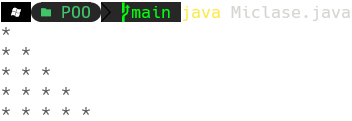
\includegraphics[width=0.75\columnwidth, center]{Pa.png}
    \end{figure}

    \subsection*{Ejercicio Práctico en el Lab}
    Realizar un programa que imprima una pirámide usando el símbolo * con base aleatoria entre 1 y 10.

    \linejump
    \textbf{Código}
    \begin{lstlisting}
import java.util.Random;

public class Piramide {
    public static void main(String[] args) {
        Random rand = new Random();

        int b = rand.nextInt(10)+1;
        int espacio = b;
        
        for(int i = 1; i <= b; i ++) {
            for(int j = 0; j < espacio; j ++)
                System.out.print(" ");            
            espacio --;

            for(int k = 0; k < i; k ++ )
                System.out.print("* ");
            System.out.println(" ");
        }
    }
}
    \end{lstlisting}

    \textbf{Terminal}
    \begin{figure}[ht]
        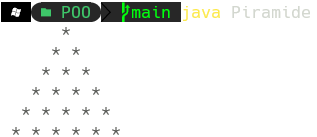
\includegraphics[width=0.75\columnwidth, center]{Pb.png}
    \end{figure}

    \section*{Resultados}
    \subsection*{Problema 1}
    Elabore un programa cuya salida sea:

    Cuando $m = 4$ ($m$ sea un numero par)
    \begin{figure}[ht]
        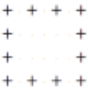
\includegraphics[width=0.25\columnwidth, center]{Cuadrado1.png}
    \end{figure}
    
    Cuando $m = 5$ ($m$ sea un numero impar)
    \begin{figure}[ht]
        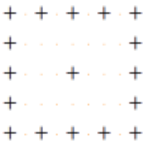
\includegraphics[width=0.25\columnwidth, center]{Cuadrado2.png}
    \end{figure}
    
    \linejump

    Donde $m$ es un número aleatorio entre 1 y 20, y cada número para imprime un cuadrado de base $m$ y cuando es impar de manera extra coloca el centro de la figura

    \textbf{Explicación} 

    Este programa crea un patrón en forma de cuadrado utilizando el carácter ``+'' y espacios en blanco. El tamaño del cuadrado se determina con un número aleatorio ``m'' entre 1 y 20. Si ``m'' es impar el boolean ``flag'' obtiene el valor de ``true''. Las líneas superior e inferior del cuadrado están formadas por caracteres ``+'', mientras que las líneas intermedias se controlan con un ciclo For para colocar espacios y los caracteres ``+'' en los lados de la figura. El ``+'' al centro se coloca con una condicional que es verdadero si se encuentra en la línea de en medio vertical y horizontal a la vez mientras ``flag'' sea verdadero.

    \textbf{Código}
    \begin{lstlisting}
import java.util.Random;

public class Cuadrado {
    public static void main(String[] args) {
        Random rand = new Random();

        int m = rand.nextInt(20) + 1;
        boolean flag;

        if(m % 2 == 0) 
            flag = false;
        else
            flag = true;

        for(int i = 0; i < m; i ++) {
            if (i == 0 || i == m - 1) {
                for(int j = 0; j < m; j ++)
                    System.out.print("+ ");
                System.out.println("");
            } else {
                System.out.print("+");

                for(int j = 0; j < (m - 2)*2 + 1; j ++) {
                    if (i == m / 2 && flag == true && j == m - 2)
                        System.out.print("+");
                    else
                        System.out.print(" ");
                }

                System.out.println("+");
            }
        }
    }
}  
    \end{lstlisting}

    \textbf{Terminal}
    \begin{figure}[ht]
        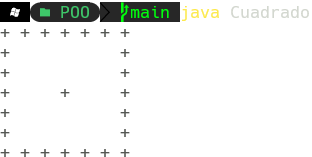
\includegraphics[width=0.75\columnwidth, center]{P1.png}
    \end{figure}


    \subsection*{Problema 2}
    Elabore un programa que reciba el del teclado un numero entero positivo mayor que 1, $k$ y realice un rombo cuya diagonal menor sea de tamaño $k$

    Ejemplo $k = 4$
    \begin{figure}[ht]
        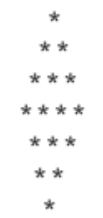
\includegraphics[width=0.2\columnwidth, center]{Rombo.png}
    \end{figure}

    \textbf{Explicación} 

    Utiliza la clase Scanner y el método ``nextInt'' se solicita al usuario un número mayor que 1. Estando dentro de un ciclo ``do while``Se realiza una comprobación por medio de un ``if'' para asegurarse de que el número ingresado sea válido y solo se sale del ``do while'' hasta que se ingrese un número valido. Luego, el programa genera un patrón en forma de rombo utilizando bucles for anidados. La primera mitad del rombo consiste en aumentar el número de asteriscos por fila, mientras que la segunda mitad disminuye el número de asteriscos por fila. Entre cada fila de asteriscos, se imprime una cantidad correspondiente de espacios en blanco para que los asteriscos formen un patrón de rombo.

    \textbf{Código}
    \begin{lstlisting}
import java.util.Scanner;

public class Rombo {
    public static void main(String[] args) {
        Scanner scanner = new Scanner(System.in);
        int k;

        do {
            System.out.print("Ingrese un numero mayor que 1: ");
            k = scanner.nextInt();
            
            if (k <= 1) 
                System.out.println("Valor Invalido\n");
        } while(k <= 1);
        scanner.close();
        
        for (int i = 1; i <= k; i++) {
            for (int j = k - i; j > 0; j--) {
                System.out.print(" ");
            }
            
            for (int j = 1; j <= i; j++) {
                System.out.print("* ");
            }
            
            System.out.println();
        }
        
        for (int i = k - 1; i >= 1; i--) {
            for (int j = k - i; j > 0; j--) {
                System.out.print(" ");
            }
            
            for (int j = 1; j <= i; j++) {
                System.out.print("* ");
            }
            
            System.out.println();
        }
    }
}
    \end{lstlisting}

    \textbf{Terminal}
    \begin{figure}[ht]
        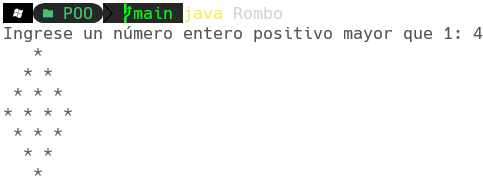
\includegraphics[width=0.75\columnwidth, center]{P2.png}
    \end{figure}

    \subsection*{Problema 3}
    Realice un programa que reciba de entrada (de tipo Scanner) de 2 a 6 números enteros positivos y determinar quién es el menor, el de en medio y el mayor. Los números que se reciban serán de uno a uno, ósea de manera secuencial.

    Ejemplo, se la entrada $\longrightarrow 4 ,2, 9, 100, 89, 3$
    
    \linejump
    Salida:
    
    \linejump
    Mayor: 100 \\
    Menor: 2 \\
    Mediana: 4

    \textbf{Explicación} 

    Este interactúa con el usuario mediante la clase Scanner para obtener la cantidad de números que se ingresarán (entre 2 y 6). Luego, solicita al usuario que ingrese los números. A medida que se ingresan los números, el programa los ordena de manera ascendente y almacena el máximo, el mínimo y la mediana de los números ingresados, de acuerdo con la cantidad de números especificada. Después de organizar los números y calcular los valores requeridos, el programa imprime el máximo, el mínimo y la mediana.

    \textbf{Código}
    \begin{lstlisting}
import java.util.Scanner;

public class MayorMenorMedio {
    public static void main(String[] args) {
        Scanner scanner = new Scanner(System.in);

        int nNumeros = 0;

        System.out.println("Cuantos numeros desea ingresar? (2 - 6)");
        while (nNumeros < 2 || nNumeros > 6) {
            nNumeros = scanner.nextInt();
            if (nNumeros < 2 || nNumeros > 6) {
                System.out.println("Error, ingrese nuevamente:");
            }
        }

        int n1 = 0, n2 = 0, n3 = 0, n4 = 0, n5 = 0, n6 = 0, tmp = 0;

        System.out.println("Ingrese los numeros:");
        n1 = scanner.nextInt();
        tmp = n1;
        n2 = scanner.nextInt();
        if (n2 < tmp) {
            n1 = n2;
            n2 = tmp;
        }
        tmp = n2;
        n3 = (nNumeros > 2) ? scanner.nextInt() : 0;
        if (n3 < tmp && nNumeros > 2) {
            n2 = n3;
            n3 = tmp;
            if (n2 < n1) {
                tmp = n1;
                n1 = n2;
                n2 = tmp;
            }
        }
        tmp = n3;
        n4 = (nNumeros > 3) ? scanner.nextInt() : 0;
        if (n4 < tmp && nNumeros > 3) {
            n3 = n4;
            n4 = tmp;
            if (n3 < n2) {
                tmp = n2;
                n2 = n3;
                n3 = tmp;
                if (n2 < n1) {
                    tmp = n1;
                    n1 = n2;
                    n2 = tmp;
                }
            }
        }
        tmp = n4;
        n5 = (nNumeros > 4) ? scanner.nextInt() : 0;
        if (n5 < tmp && nNumeros > 4) {
            n4 = n5;
            n5 = tmp;
            if (n4 < n3) {
                tmp = n3;
                n3 = n4;
                n4 = tmp;
                if (n3 < n2) {
                    tmp = n2;
                    n2 = n3;
                    n3 = tmp;
                    if (n2 < n1) {
                        tmp = n1;
                        n1 = n2;
                        n2 = tmp;
                    }
                }
            }
        }
        tmp = n5;
        n6 = (nNumeros > 5) ? scanner.nextInt() : 0;
        if (n6 < tmp && nNumeros > 5) {
            n5 = n6;
            n6 = tmp;
            if (n5 < n4) {
                tmp = n4;
                n4 = n5;
                n5 = tmp;
                if (n4 < n3) {
                    tmp = n3;
                    n3 = n4;
                    n4 = tmp;
                    if (n3 < n2) {
                        tmp = n2;
                        n2 = n3;
                        n3 = tmp;
                        if (n2 < n1) {
                            tmp = n1;
                            n1 = n2;
                            n2 = tmp;
                        }
                    }
                }
            }
        }
        scanner.close();

        int maximo = 0;
        if (nNumeros == 6) {
            maximo = n6;
        } else if (nNumeros == 5) {
            maximo = n5;
        } else if (nNumeros == 4) {
            maximo = n4;
        } else if (nNumeros == 3) {
            maximo = n3;
        } else if (nNumeros == 2) {
            maximo = n2;
        }
        int minimo = n1;
        int mediana = 0;

        if (nNumeros == 2) {
            mediana = (n1 + n2) / 2;
        }
        else if (nNumeros == 3) {
            mediana = n2;
        }
        else if (nNumeros == 4) {
            mediana = (n2 + n3) / 2;
        }
        else if (nNumeros == 5) {
            mediana = n3;
        }
        else if (nNumeros == 6) {
            mediana = (n3 + n4) / 2;
        }    
        
        System.out.println("Maximo: " + maximo);
        System.out.println("Minimo: " + minimo);
        System.out.println("Mediana: " + mediana);
    }
}
    \end{lstlisting}

    \textbf{Terminal}
    \begin{figure}[ht]
        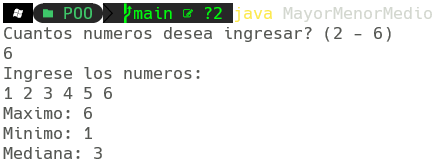
\includegraphics[width=0.75\columnwidth, center]{P3.png}
    \end{figure}

    \subsection*{Problema 4}
    Programar ``War of Numbers'' el ejercicio de describe en: \\
    \url{https://edabit.com/challenge/7fHsizQrTLXsPWMyH}

    Sólo que, en lugar de recibir un arreglo de enteros, la guerra sea con 10 números aleatorios entre 1-1000

    \textbf{Explicación} 
 
    Este programa utiliza la clase Random para generar 10 números aleatorios entre 1 y 1000 y mediante una condicional separa los pares de los impares para sumarlos por separado. Luego compara que suma es mayor y le resta la otra para guardar la diferencia en la variable ``diff''. Finalmente imprime a consola los numero aleatorios, las sumas y la diferencia.

    \textbf{Código}
    \begin{lstlisting}
import java.util.Random;

    public class WarOfNumbers {
    public static void main(String[] args) {
        Random rand = new Random();

        int number, evenSum = 0, oddSum = 0, diff;

        System.out.print("Numeros: ");
        for(int i = 0; i < 10; i ++) {
            number = rand.nextInt(1000) + 1;
            System.out.print(number + " ");
            
            if (number % 2 == 0) 
                evenSum += number;
            else 
                oddSum += number;
        }

        System.out.println("\nSuma de pares: " + evenSum);
        System.out.println("Suma de impares: " + oddSum);

        if(evenSum >= oddSum)
            diff = evenSum - oddSum;
        else 
            diff = oddSum - evenSum;

        System.out.println("Diferencia: " + diff);
    }
}            
    \end{lstlisting}

    \textbf{Terminal}
    \begin{figure}[ht]
        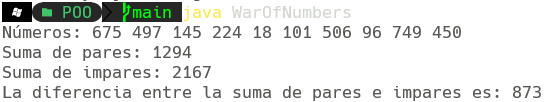
\includegraphics[width=0.75\columnwidth, center]{P4.png}
    \end{figure}


    \subsection*{Problema 5}
    Programar el problema descrito en: \\
    \url{https://edabit.com/challenge/4r33Yd2HuEireb3Sm}

    \textbf{Explicación} 

    El siguiente programa utiliza la clase Random para generar un número aleatorio entre 1 y 10000. Luego, el programa determina la cantidad de dígitos en ese número. Para hacerlo, inicializa una variable llamada ``digitCount'' en 0 y crea una copia del número generado para no modificar el valor original. Luego, emplea un condicional para verificar si el número es 0; en ese caso, le asigna 1 al contador de dígitos. Si el número no es 0, utiliza un bucle ``while'' para dividir sucesivamente el número entre 10 y, al mismo tiempo, incrementar el contador de dígitos hasta que el número se vuelva 0. Finalmente, imprime el número aleatorio generado y la cantidad de dígitos que tiene.

    \textbf{Código}
    \begin{lstlisting}
import java.util.Random;

public class IntegerDigitsCount {
    public static void main(String[] args) {
        Random random = new Random();

        int randomNumber = random.nextInt(10000) + 1;
        int digitCount = 0;
        int number = randomNumber;
        
        if (number == 0) {
            digitCount = 1;
        } else {
            while (number != 0) {
                digitCount++;
                number /= 10;
            }
        }

        System.out.println("Numero generado: " + randomNumber);
        System.out.println("Cantidad de digitos: " + digitCount);  
    }  
}
    \end{lstlisting}

    \textbf{Terminal}
    \begin{figure}[ht]
        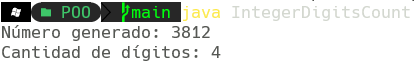
\includegraphics[width=0.75\columnwidth, center]{P5.png}
    \end{figure}


    \section*{Conclusiones}
    Al llevar a cabo esta práctica, hemos logrado reconocer los componentes fundamentales que conforman el lenguaje de programación Java. Estos elementos juegan un papel crucial en su funcionamiento y pertinencia en el ámbito de la programación. La colaboración entre estos conceptos, como la Máquina Virtual de Java (JVM), el Java Development Kit (JDK), la codificación y la compilación, sienta las bases en las cuales podemos edificar soluciones para desafíos tecnológicos.


    \section*{Referencias}
    \small
    Jacob E. \textit{War of Numbers}. Edabit. \url{https://edabit.com/challenge/7fHsizQrTLXsPWMyH} \\

    Xavier D. \textit{Integer Digits Count}. Edabit \url{https://edabit.com/challenge/4r33Yd2HuEireb3Sm}
\end{document}